\Chapter{Tervezés}

Itt kezdődik a dolgozat lényegi része, úgy értve, hogy a saját munka bemutatása.
Jellemzően ebben szerepelni szoktak blokkdiagramok, a program struktúrájával foglalkozó leírások.
Ehhez célszerű UML ábrákat (például osztály- és szekvenciadiagramokat) használni.

Amennyiben a dolgozat inkább kutatás jellegű, úgy itt lehet konkretizálni a kutatási módszertant, a kutatás tervezett lépéseit, az indoklást, hogy mit, miért és miért pont úgy érdemes csinálni, ahogyan az a későbbiekben majd részletezésre kerül.

Ebben a fejezetben az implementáció nem kell, hogy túl nagy szerepet kapjon.
Ez még csak a tervezési fázis.
(Nyilván ha olyan a téma, hogy magának az implementációnak a módjával foglalkozik, adott formális nyelvet mutat be, úgy a kódpéldákat már innen sem lehet kihagyni.)

\Section{RDF használata}
Az esetünkben felhasznált adatok ábrázolására a következőképpen nézne ki az RDF modell. Az akkord reprezentálná a hármasok közül a témát, vagyis a subject-et, mivel azt kellene először definiálni. Az akkord, ami más néven hármas hangzat, alapvetően három hangból épül fel. Van a fő hang, ami tegyük fel, ha C-dúr akkordot akarunk modellezni, az a C hang lesz, erre épül a dúr esetében a nagy terc, ami az E hangot fogja adni, valamint a C hanghoz igazított kvint távolságra levő G hang. Tehát a C-dúr akkordot a C E és G hangokból lehet összeállítani, ezek egyben fokok is, amiket predikátumként fogunk jelölni, hogy melyik hang az akkord hanyadik foka. Ezt a következő ábrán lehet látni.
\begin{figure}[h]
	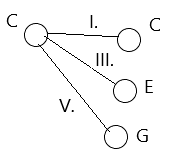
\includegraphics[scale=1]{images/rdf_graph.png}
	\caption{Szemantikai ábrázolás az RDF szerint.}
	\label{fig:graph1}
\end{figure}
Az ábrán látható, hogy egy akkord meghatározásához 3 él vezet kifelé, ugye ezek jelzik, hogy melyik fokon található a C-dúr akkord hangjai (rendre I., III. és V. fok ) és az objektumok maguk a hangok, ahova az él mutat. Ebben az esetben meg is lenne oldva az akkordok reprezentálása RDF modell szerint, viszont a kottába való visszahelyezéskor a programnak szükséges tudnia azt is, hogy pontosan hova illessze vissza a megfelelő akkordot egy transzponálás esetében, mikor is a hangnem változik, és a kottába szereplő akkordok kicserélődnek. 
Ilyenkor szintén használva a gráf elméletét az akkord alatti szövegrész lesz az objektum az él pedig elnevezve a pozíció lesz. Ugyanis a kottában szereplő szöveg nem változik ugye csak az akkordok, ha bármilyen művelet kerül végrehajtásra. Többféle probléma merülhet fel, abban az esetben, ha statikusan akarom használni a doboz-t amit az akkordhoz kivág a program a szöveggel együtt, akkor annak a méretét egy kalkulált értékből kell kapnia, ami illeszkedik a megfelelő felbontáshoz, mert hogy a felbontás különböző egyes kották képeinél.

\Section{Tesseract használata}
A tesseract nevezetű ocr szoftvert használom a karakterfelismerésre a dolgozatban, nevezetesen a pytesseract függvénykönyvtárat. Ez alapvetően a Google OCR motorja, amit implementáltak python környezetben. Önmagába álló szkriptként is használható, és széles körben felismer különböző kiterjesztésű képeket, mint például a jpeg, png, gif, bmp, tiff és egyéb másokat, habár ugyanúgy megvannak a korlátai is, amiről majd később térek ki részletesebben. Elsőként mivel hogy különálló maga a program ezért PATH-ba kellett helyezni, amivel sajnos meggyűlt a baj, mivel hogy nem ismerte fel az operációs rendszer. Így a következőképpen oldottam meg, hogy használható legyen:
\begin{python}
import pytesseract
	
local_path =  r'C:\Program Files\Tesseract-OCR\tesseract.exe'
pytesseract.pytesseract.tesseract_cmd = local_path
\end{python}
A lokális környezetbe való fejlesztés erejéig volt használatba ez az elérési útvonal. A függvénykönyvtárnak az image to string nevű metódusát használtam arra, hogy a képből szöveg váljon. Paraméterként megadható, hogy ugye mely képekből kell a szöveget kiolvasni, és többek között, amit használtam én is az a nyelv megadása, valamint konfigurációt is meg tudtam adni. A pontosság az elején zavaró volt, mert túlságosan zajos volt a kép sokszor, ahhoz, hogy az OCR megfelelően ki tudja venni, hogy mely karakterről is van szó. Ehhez az egyik megolás az volt, hogy jobban lehessen manipulálni a bemeneti képet, amivel dolgozik a Tesseract.
\newpage
\Section{Szemantikus ábrázolás RDF-el}

\begin{figure}[h]
	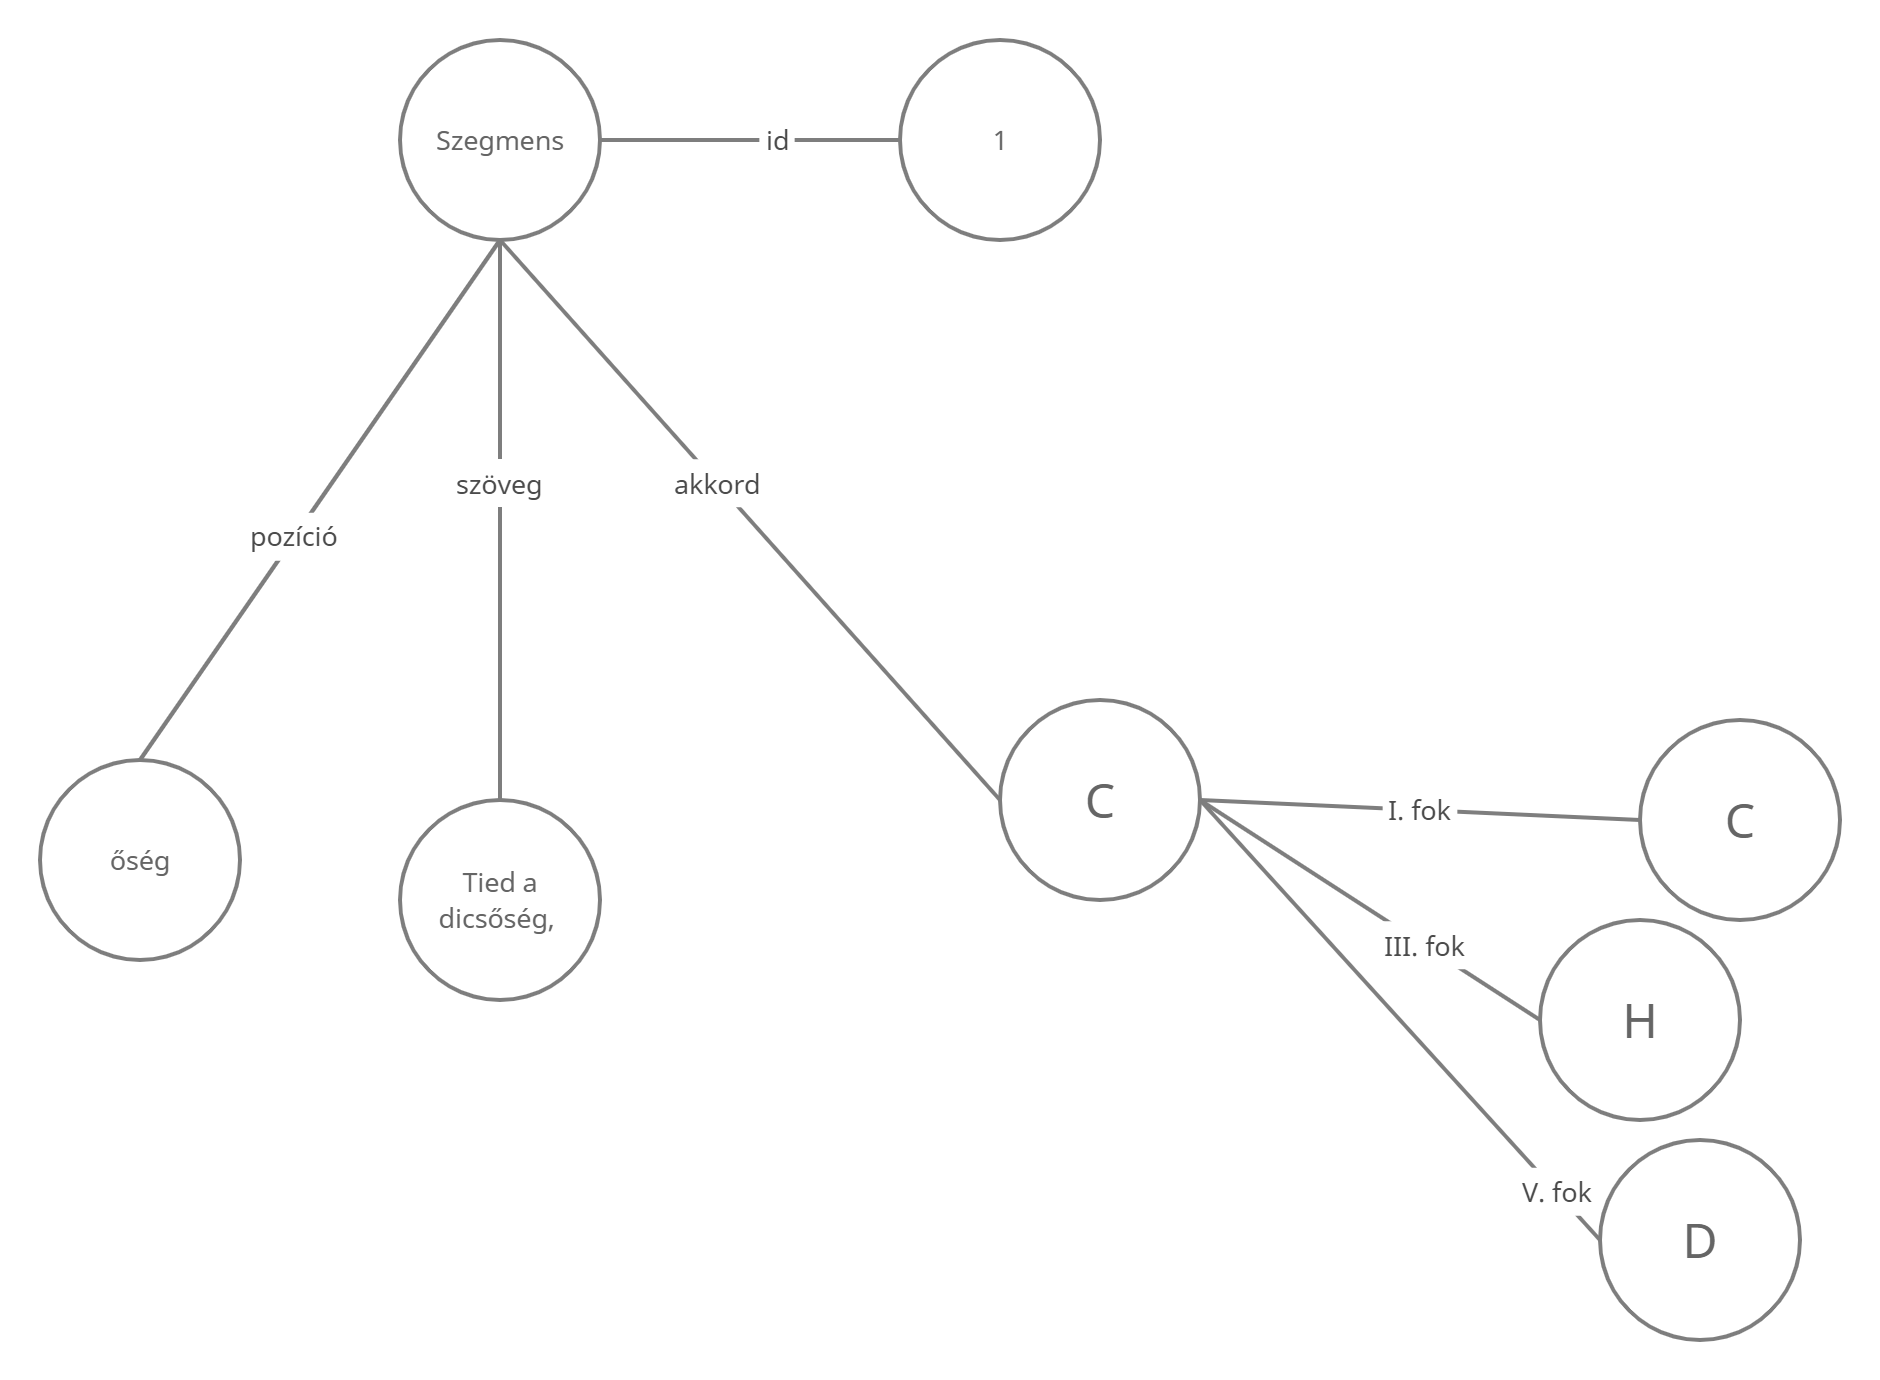
\includegraphics[scale=0.2]{images/rdf_graph_2.png}
	\caption{Konkrét szemantikai ábrázolása a dalnak.}
	\label{fig:graph2}
\end{figure}

A 3.2-es ábrán látható, hogy az adott példa kottánkban hogy nézne ki egy szegmens. A szegmens most jelen esetben az akkord és az ahhoz tartozó szöveg leírása. A jelenlegi kottához 19 db ilyen szegmens tartozik, indexelve az akkord alapján, tehát 19 akkord van a dalban. A kiinduló elemből az első elágazás az id-hoz vezet, nagyon egyszerűen, ez csak az azonosító száma a dalban szereplő szegmensnek. Ezek alapján például úgy csináltam meg a programot, hogy egy tömb adatstruktúrába adtam meg neki, hogy melyik szegmensnél történik a sortörés, és azoknál a szegmenseknél belefut a program egy plusz ágba, ahol sortörés és a változók újrainicializálása történik. Onnantól következik a pozíció, ami azt a szövegrészt tárolja a szegmensből, ami egyedien azonosítja, hogy az akkord pontosan hol helyezkedik el a szegmensben, egyenlőre ez egy változó hosszúságú string, de érdemes meghatározni, hogy 3 esetleg 4 hosszúsággal történjen ugye a kiolvasás a következetesség szempontjából. A következő elágazás a szövegre mutat, tehát ami konkrétan benne lesz majd a végkifejletbe, ebből származik a pozíció, amiről fentebb szó volt már. Ezután következik az akkord, ami a jelenlegi ábrázolásba úgy néz ki, hogy a szegmens akkordja az egy C, viszont a tonika az külön meghatározandó, vagyis, hogy dúr vagy mol az adott akkord. Az akkordból 3 predikátum mutat objektumokra és ez az amiből felépül egy akkord. Az első fok mutat az alaphangra, a harmadik a tercére az alaphangnak, amiből megállapítható, hogy mol vagy dúr az akkord, mert ha mol, akkor az alaphangra épített kis tercről van szó ami jelen esetben nem így van, hiszen a C - re épített nagy terc a G hang, tehát ez az akkord dúr. És a harmadik objektum az ötödik fok, tehát az alaphang, vagyis a C hang tiszta kvintre levő távolsága, azaz a H hang.

 J\Section{Kotta tárolási példák}
\SubSection{Music XML}
\begin{xml}
<?xml version="1.1" encoding="UTF-8" standalone="no"?>
<!DOCTYPE score-partwise PUBLIC
"-//Recordare//DTD MusicXML 1.1 Partwise//EN"
"http://www.musicxml.org/dtds/partwise.dtd">
  <score-partwise>
    <part-list>
      <score-part id="P1">
        <part-name>Music</part-name>
      </score-part>
    </part-list>
    <part id="P1">
      <measure number="1">
        <attributes>
          <divisions>1</divisions>
          <key>
            <fifths>0</fifths>
          </key>
          <beats>4</beats>
          <beat-type>4</beat-type>
          <clef>
            <sign>G</sign>
            <line>2</line>
          </clef>
        </attributes>
        <note>
          <pitch>
            <step>C</step>
            <octave>4</octave>
          </pitch>
          <duration>4</duration>
          <type>whole</type>
        </note>
      </measure>
    </part>
  </score-partwise>
\end{xml}

Ez a MusicXML egyik példája, a kotta tárolására. Mivel a minta adat, tehát az itt jelenlevő kották másképpen épülnek fel, ahogy az feljebb is említésre került, így egy saját xml valahogy így nézne ki

\SubSection{Saját kottatárolási módszer XML-ben}
\begin{xml}
<?xml version="1.1" encoding="UTF-8" standalone="no"?>
  <sheet>
    <key>
      <note>C</note>
      <chord>major</chord>
    </key>
    <segment id="1">
      <note>C</note>
      <text>Tied a dicsőség, </text>
      <position>őség</position>
    </segment>
    <segment id="2">
      <note>em7</note>
      <text>és imádás,\n</text>
      <position>im</position>
    </segment>
    <segment id="3">
      <note>F</note>
      <text>Felemeljük </text>
      <position>elj</position>
    </segment>
    <segment id="4">
      <note>dm</note>
      <text>kezeinket\n</text>
      <position>in</position>
    </segment>
    <segment id="5">
      <note>F/G</note>
      <text>És dicsérjük </text>
      <position>csé</position>
    </segment>
    <segment id="6">
      <note>G</note>
      <text>szent neved!\n</text>
      <position>ved</position>
    </segment>
    <segment id="7">
      <note>G7</note>
      <text>Ó, Hatal</text>
      <position>Hat</position>
    </segment>
    <segment id="8">
      <note>C</note>
      <text>mas, </text>
      <position>mas</position>
    </segment>
    <segment id="9">
      <note>am</note>
      <text>Keze nagy csodákat tesz,\n</text>
      <position>esz,</position>
    </segment>
    <segment id="10">
      <note>F</note>
      <text>Vele senki nem ér fel</text>
      <position>fel</position>
    </segment>
    <segment id="11">
      <note>dm7</note>
      <text>, Vele </text>
      <position>, Ve</position>
    </segment>
    <segment id="12">
      <note>G</note>
      <text>senki nem ér </text>
      <position>se</position>
    </segment>
    <segment id="13">
      <note>G7</note>
      <text>fel.\n</text>
      <position>fel</position>
    </segment>
    <segment id="14">
      <note>G7</note>
      <text>Ó, Hatal</text>
      <position>Hat</position>
    </segment>
    <segment id="15">
      <note>C</note>
      <text>mas, </text>
      <position>mas</position>
    </segment>
    <segment id="16">
      <note>am</note>
      <text>ó, Hatalmas, </text>
      <position>mas</position>
    </segment>
    <segment id="17">
      <note>F</note>
      <text>ó, Hatalmas,</text>
      <position>mas</position>
    </segment>
    <segment id="18">
      <note>G7</note>
      <text> ó, Hatal</text>
      <position> ó</position>
    </segment>
    <segment id="19">
      <note>C</note>
      <text>mas!</text>
      <position>mas</position>
    </segment>
  </sheet>

\end{xml}

Szegmensekre van bontva az adott akkord és a hozzátartozó szöveg. Minden szegmens kap egy id-t ami a sortöréshez szükséges az első verzió szerint. A szegmensen belül a note tárolja az akkordot, a text a blokkhoz tartozó szöveget, a position pedig tárolja az akkord elhelyezkedését a szöveg felett. Python-ba ehhez készült egy szemléltető program, ami ezt az xml-t jeleníti meg egyenlőre konzolon.

\Section{XML beolvasás}
\SubSection{Megfigyelések}
A jelen példában 3 részre van bontva a kotta, szöveg, akkord, pozíció. Ahhoz, hogy ebből tudjon  működni a konzolra kiiratás a megfelelő pozíciókkal, az indexelést tettem lista adatstruktúrába, hogy meglegyen mindegyik akkordnak a megfelelő pozíciója. Kétfajta adat kerül tárolásra, az egyik mindenképpen az, hogy az xml-ben megadott string alapján melyik indexű karakternél található a szegmens szövegében a string maga, mert az jelöli az akkord helyét. A másik pedig maga a string ami kiadja a kotta véglegesítését, a konkatenált akkord, - és szóközszámmal, valamint a kotta szövegével.

Az első elakadást az egy sorba történő többszöri előfodulású szöveg okozta, amit úgy oldottam meg, hogy ha már egyszer megtalálható a sorban az adott substring, akkor azt megszámolja hányszor fordul elő, annyiszor kihagyja azt és a következőt vegye számításba az indexelésnél. Ehhez tartozik a számláló, ami olyan értéket kap, amennyi előfordulása van a substringnek az addig befűzött sorba.

A beolvasás célja egyenlőre csak az, hogy a kotta kikerüljön a konzolra, lényegében, ha transzponálási műveletet akarunk végrehajtani a kottán, akkor ennél részletesebben szükséges megadni az akkordot. Ugye, ahogy fentebb is írtam, az akkord hármashangzatba(vagy négyeshangzat, a jelölésektől függően) gondolva alapjáraton az első a harmadik és az ötödik fokból áll, amikor dúrról beszélünk. Ehhez már szükséges, akkor az, hogy az xml létrehozásakor külön legyen választva a mol és a dúr is. Egységesen meg van oldva ez az összes kottára nézve, ami mol akkordokat jellemzik, azok a következők:
\begin{itemize}
\item[--]az akkord kisbetűvel van
\item[--]az akkord kisbetűvel van és mellette egy kis m betű áll (pl.: am egy a-molt jelöl)\linebreak
\end{itemize}
Ami pedig a dúr akkordokat jellemzik:
\begin{itemize}
	\item[--]az akkord nagybetűvel van
\end{itemize}
	
Ezeket amikor képes megkülönböztetni a program, akkor ennek megfelelően fogja tudni lementeni a note mellé azt a property-t ami jelöli, hogy az akkord az mol vagy dúr. Legyen a neve mondjuk tone. Ebből kiindulva így nézne ki az egyik szegmens:
\begin{xml}
<segment id="12">
  <chord>
    <note>G</note>
    <tone>major</tone>
  </chord>
  <text>senki nem ér </text>
  <position>se</position>
</segment>
\end{xml}

Miután meg lehet különböztetni a mol-t a dúrtól, ezután mivel akkordról beszélünk, ami legtöbb esetben hármas hangzat, azt is fel kell osztani. Az akkord a hang diatonikus I. III. és V. fokából épül fel, valahogy így nézne ki, ha letárolnánk xml adatstruktúrába csak egy szegmensét:
\begin{xml}
<segment id="12">
  <chord>
    <note>G</note>
    <measures>
    	<I>G</I>
    	<III>H</III>
    	<V>D</V>
    </measures
    <tone>major</tone>
  </chord>
  <text>senki nem ér </text>
  <position>se</position>
</segment>
\end{xml}


\Section{További környezetek}

A matematikai témájú dolgozatokban szükség lehet tételek és bizonyításaik megadására.
Ehhez szintén vannak készen elérhető környezetek.

\begin{definition}
Ez egy definíció
\end{definition}

\begin{lemma}
Ez egy lemma
\end{lemma}

\begin{theorem}
Ez egy tétel
\end{theorem}

\begin{proof}
Ez egy bizonyítás
\end{proof}

\begin{corollary}
Ez egy tétel
\end{corollary}

\begin{remark}
Ez egy megjegyzés
\end{remark}

\begin{example}
Ez egy példa
\end{example}
